\chapter{Introduction}


%\rod{Noter til afsnittet: Fokus på vand som scarce resource, kun på det vi skal bruge, mere smooth introduktion til CT.}

Freshwater is becoming an increasingly scarce resource %\citep{altmanMembraneTreatmentSidestream2012}%
, by 2025 WHO estimate that half the world's population will live in areas where demand for water exceeds the supply. \citep{WHO2017} 
Industrial processes use up a large quantity of the world's freshwater supply  \citep{koemanMembraneDistillationIndustrial2016}. 
As the supply of freshwater declines, costs and competition for the resource is expected to rise \citep{altmanMembraneTreatmentSidestream2012}, making it more important to close water cycles and relieve the environment of water stress \citep{koemanMembraneDistillationIndustrial2016}.
%This project will investigate the reducing in water usage in an ongoing collaboration with Grundfos. 
Grundfos, a major Danish company which provides water solutions, have proposed to reduce water usage in cooling towers (CT), as a part of their focus on sustainability. 
CTs are industrial processes which are responsible for up to 60-70 \% of total freshwater usage in industry \citep{koemanMembraneDistillationIndustrial2016} \citep{farahanniRecoveryCoolingTower_2016}. 
%This project will therefore be performed in collaboration with Grundfos' focus on reducing water usage in cooling towers. 
%CT which constitute 60-70 \% of the total freshwater consumption in industry. \citep{koemanMembraneDistillationIndustrial2016}.
CTs remove excess heat by continuously recirculating and evaporating water from a reservoir. 
This continuous loss of water leads to scaling and corrosion problems as species are concentrated in the water reservoir.
\citep{PlantEngineerBookReference2001}. 
Membrane technology has been proposed as a viable option for treatment of wastewater from cooling towers, potentially reducing water usage, and closing the water cycle. \citep{kaliappan_RecoveryReuseWater_2005}
%This project will therefore be performed in collaboration with Grundfos, with focus on reducing water usage in cooling towers by membrane filtration. 


%Grundfos has proposed a filtration system using Nano Filtration (NF) to treat and thus recycle waste water from cooling towers using inside-out hollow-fiber membranes. 



\section{Membrane Filtration for Reducing Water Usage}
% \rod{intro af sammenarbejde med GF, kort intro til CT, ref til billede, NF case studies ref til billede. }

%Grundfos has proposed a filtration system using Nano Filtration (NF) to treat and thus recycle wastewater from cooling towers using inside-out hollow-fiber membranes. 


%Previously waste water from CT was simply discharged to surface water without treatment leading to environmental contamination \citep{farahanniRecoveryCoolingTower_2016}
%Water scarcity and increasing water prices have been motivation for research in reusing water for CT. \citep{farahanniRecoveryCoolingTower_2016}. 
Multiple technologies have been investigated to assess their potential as tools to reduce water usage of CTs.
Typically, they are aimed at reducing the concentration of various species present in the CT system e.g., by side-stream treatment. %mangler lige en kilde
Apart from decreasing water usage there are other important factors to consider when treating water for CTs: maintaining operation efficiency, protecting the CT equipment, environmental impacts, and chemical cost. \citep{IntroductionCoolingTower2014}
Under traditional CT operation large quantities of water is led to the drain to mitigate the steadily increasing concentrations of various species caused by the loss of pure water as evaporation from the reservoir, see \cref{fig:CT_working_principle}.
This process is typically called 'blowdown' (BD) and may be a continuous process or occur only when signal values exceed limit values. \citep{PracticalApproachWater2007}
By replacing evaporated water and BD with freshwater of higher quality i.e., 'make-up' water (MU), normal operation of the CT can be maintained.
\citep{IntroductionCoolingTower2014}

Membrane filtration has been shown to be a potential route for the reduction of water usage in CTs.  
%Membrane filtration has been widely used for desalination in other areas.  
Typically pressure driven membrane processes are microfiltration (MF),
ultrafiltration (UF), nanofiltration (NF), and reverse osmosis (RO), listed in order from lowest to highest removal efficiencies. 
These processes utilise an applied pressure as a driving force in the separation of a fluid stream over a semipermeable membrane. 
During side-stream filtration the BD stream is treated and permeate is returned to the CT reservoir, thus reducing the amount of make-up water needed along with the volume of BD, discharged to the drain \cite{farahanniRecoveryCoolingTower_2016}, see \Cref{fig:CT_working_principle}.
The different membrane types typically have differing characteristics and fields of application, however for some types there are less clear boundaries e.g., NF can be seen as a mixture between UF and RO processes.\citep{keo}
NF is generally able to retain multi-valent ions but monovalent ions only to a lesser degree. \citep{keo}
The ability of NF membranes to retain most species while typically having lower energy requirements is what makes it well suited for use in CT side-stream filtration.  \citep{farahanniRecoveryCoolingTower_2016} 

\begin{figure}[H]
    \centering
    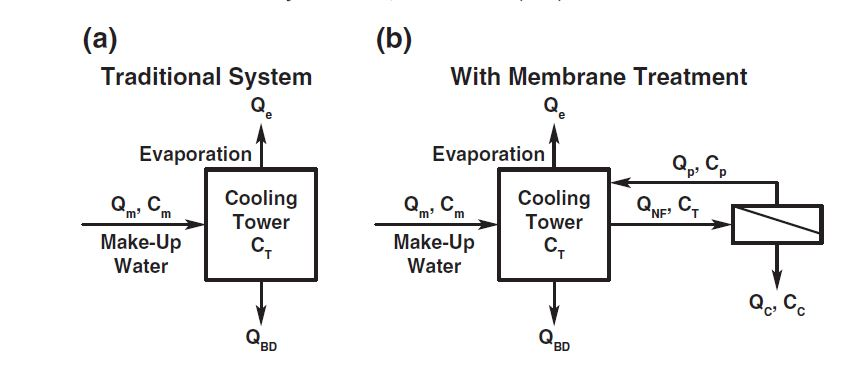
\includegraphics[width=1\textwidth]{Billeder/intro/CT_CTandNF.JPG}
    \caption{\citep{altmanMembraneTreatmentSidestream2012} Illustration of side-stream treatment of CTs by membrane technology}
    \label{fig:CT_working_principle}
\end{figure}



This viability was tested in a study by Altman et al. 2012 where a pilot-scale experiment used NF to treat the BD stream of a CT  \citep{altmanMembraneTreatmentSidestream2012}.
The experiment ran for three months and found that the maximum water savings for the CT were 16\% and 49\% for the make-up and blowdown respectively.
The actual water saving was much lower due to high degree of scaling on the membranes, primarily due to silica and calcium salts. 
The membrane performance was 89-99\% removal of dissolved constituents. \citep{altmanMembraneTreatmentSidestream2012} 
This is in good agreement with another study by Kaliappan et al. 2005 which also used NF to treat a CT BD stream. \citep{kaliappan_RecoveryReuseWater_2005}
They found salt rejections of 87 - 89 \%.
It was noted that such high rejections are unnecessary and that membranes with lower rejection rates (70-90\%) but higher water recoveries would better suit use with CTs. \citep{kaliappan_RecoveryReuseWater_2005}
Both studies also noted fouling as a major problem. \citep{altmanMembraneTreatmentSidestream2012}  \citep{kaliappan_RecoveryReuseWater_2005}


There have also been multiple studies on implementing RO membranes in the same manner for treatment of CT BD.
Using discarded RO membranes for treatment of BD stream have been investigated by Frick et al. 2014.  
They were deemed appropriate for CT BD filtration as characterization of the discarded RO membranes determined their performance to be similar to NF membranes. \citep{frickEvaluationPretreatmentsBlowdown2014}.
A study by Farahanni et al. 2016  investigated and compared RO and NF filtration for the purpose of recovering water from CT BD streams along with evaluating different pre-treatments. \citep{farahanniRecoveryCoolingTower_2016}
The RO membrane showed better rejection of TDS and COD removal; however, it was commented that increased operational costs of RO membranes make them difficult to recommend over NF for use as side-stream treatment in CTs.
Both RO and NF systems required pre-filtration to avoid fouling and it was generally apparent that the RO membranes required a more thorough pre-filtration to make them viable.  \citep{farahanniRecoveryCoolingTower_2016}
%Coagulation/flocculation was shown to be the most efficient method increasing permeate flux by 25\% and 33\% for NF and RO respectively.
%Using MF or UF membranes as pre-treatment options for BD treatment was investigated in \citep{zhangPilotTestingOutsidein2007,zhangPilotTestUF2008}  
%Other types of technologies often implemented in desalination have also been investigated in regards to treatment of CT wastewater.
%\textbf{Liao et al.} and \textbf{Silvia Lucila et al.} used electrocoagulation to remove ions. 
Mainly silica and calcium were deemed the most troublesome ions for CT operation from cooling tower BD water \citep{liaoTreatmentCoolingTower2009}, 
generally the water quality in a CT system is critical for operation efficiency and longevity \citep{IntroductionCoolingTower2014}.


\section{Water Quality}

%\rod{vand kvalitet, introducer COC som operation factor, fokus på solubility af salte, udregn noget COC, hvilke problemer der er med vandet. name drop ion balancen (i forhold til Na).}
The quality of cooling water should be considered and maintained in order to avoid corrosion, scaling and solid deposition within the tower.  \citep{IntroductionCoolingTower2014}
%The water quality in a CT system is critical for operation efficiency and longevity \citep{IntroductionCoolingTower2014}. 
%The maximum allowable concentrations in makeup water is limited by potential scaling, corrosion and fouling. \citep{PracticalApproachWater2007}.
%Therefor different CT manufactures have varied guidelines for limiting concentration of various contaminants, depending on the CT material and configuration. \citep{BAC_guidelines}, \citep{Evapco_guidelienes}.  
The primary reason for scaling is supersaturation, where salt exceed solubility limits and deposition occur. %, solubility is depending on e.g. temperature and pH 
\citep{PracticalApproachWater2007} 
The most common scale forming salt is calcium carbonate present as calcite (\ce{CaCO3}) \citep{IntroductionCoolingTower2014} \citep{PracticalApproachWater2007}. 
As the degree of scaling often depend on calcium levels a reduction of the hardness of the makeup water can be applied to combat scaling, i.e., by removing calcium e.g., by use of ion exchange or membrane filtration.  \citep{PracticalApproachWater2007}
Other common scaling minerals are %calcium phosphate,
calcium sulfate and silica  \citep{IntroductionCoolingTower2014} \citep{PracticalApproachWater2007}. 
%Silica scaling occur when silica exceed solubility limit in water, a conservative limit is often 150 ppm. 
%intro hvorfor er silica et problem. 
Silica scaling is an unsolved problem for membrane desalination techniques, as silica fouling on membranes leads to reduced flux and water recoveries, furthermore silica fouling on heat exchanges leads to limit in heat transfer and therefore decrease in energy efficiency.  \citep{ChemistrySilicaScale2014}
The major parameters that control silica solubility and reactions are pH, temperature, ionic strength, other multivalent ions, and silica concentration \citep{ChemistrySilicaScale2014}, a conservative silica limit is 150 ppm \citep{IntroductionCoolingTower2014}
Due to temperature dependency on solubility silica scaling in cooling towers would deposit first on the slats (filler material) where the temperature is lower. \citep{IntroductionCoolingTower2014}
 %but the solubility depends on temperature and pH, where higher pH gives higher solubility.  \citep{IntroductionCoolingTower2014}. 

%The degree of scaling often depend on calcium levels, bicarbonate alkalinity levels and water temperature \citep{IntroductionCoolingTower2014}
%Therefor calcium, sulphate and silica levels should be monitored to control scaling if ion exchange is used to reduce hardness sodium should also be monitored to control the charge balance. 

%Corrosion is destruction of metal by chemical or electrochemical reactions. 
%corrosion can lead to equipment faliure. 
High concentration of chloride can cause pitting corrosion, where chlorides concentrate in pits and leads to acidic environments with low oxygen. \citep{Ma12} %, leading to corrosion. \citep{Ma12} \citep{PracticalApproachWater2007}
Chloride and sulphate can also increase corrosion rate due to  increase in conductivity.
To combat corrosion pH should be monitored as acidic or slightly alkaline aqueous environments dissolves metals and protective oxide films. \citep{PracticalApproachWater2007}
Finally fouling due to suspended solids e.g., from biofilm or air-borne substances can be combated by filtration and increased velocities. \citep{PracticalApproachWater2007}
%Deposits, corrosion and biological fouling within a CT can interfere with the heat transfer and thus reduce operation efficiency and longevity. \citep{IntroductionCoolingTower2014}
Based on guidelines from CT manufactures as well as scaling and corrosion theory the parameters and species which are problematic to the operation of CTs are identified as: pH, conductivity, concentration of calcium, chloride, silica, and sulfates. 
These species are summarized in 
\cref{Tab:CT_water_threshhold} with recommend thresholds \textcolor{blue}{kilder}. 
 



%In order to avoid scaling, corrosion and fouling, CT manufactures have guidelines for limiting concentration of various contaminants, these vary depending on the CT material and configuration \citep{BAC_guidelines}, \citep{Evapco_guidelienes}. 
These guidelines are used in the operation of CTs and are based on the relationship between quality or volume of makeup and blowdown water, expressed as cycles of concentration (COC) \citep{IntroductionCoolingTower2014}. 
The COC parameter describes the total amount of minerals which are concentrated in the cooling water compared to the concentration in the makeup water, or the volume described by \cref{eq:COC_eq}. \citep{IntroductionCoolingTower2014} 
The salt or species which has the lowest calculated COC is the limiting factor controlling operation of the CT. \citep{IntroductionCoolingTower2014} \citep{PracticalApproachWater2007}. 
%, as this species will most likely be the first to scale or corrode the CT system. 


\begin{ceqn}
    \begin{align}
    \label{eq:COC_eq}%\label{eq:rejection_formula}
       COC = \frac{ Q_{MU}}{ Q_{BD}}= \frac{ C_{BD}}{C_{MU}}
    \end{align}
\end{ceqn}
Where \textit{Q} represents volume and \textit{C} concentration, %subscript MU describes CT makeup water and BD the blowdown stream. 
In order to identify the most problematic species during operation of a CT the COC is calculated based on threshold guidelines presented in \cref{Tab:CT_water_threshhold}. 
This identifies calcium and silica as the most problematic species with a $COC_{max}$ of 3 for normal CT operation. 
If silica is above 30 mg/L in the makeup water silica will most likely be the parameter which controls COC. \citep{IntroductionCoolingTower2014}

\begin{table}[h]
\centering
\caption{Threshold values and their effect on COC for example MU stream,WIP. } 
\begin{tabular}{lc|ccc}
Species            & Unit & Threshold  & Make-up & $COC_{max}$ \\ \hline
pH                  &    & 6.5-9.0   & 8 & - \\
Conductivity &[$\mu$S/cm]   & 1200     &  300   &   4   \\
Calcium   &[ppm]               & 150   &  50  &3\\
Chloride &[ppm]          & 250       & 50  &5     \\
Silica   & [ppm]              & 150       & 50    &3   \\   
Sulfates  &  [ppm]            & 250       & 50      &5 \\

\end{tabular}
\label{Tab:CT_water_threshhold}
\end{table}


%COC is also a measure of water efficiency where high water efficiency is desired achieved by high COC, a COC of 3 is acceptable water efficiency. \citep{IntroductionCoolingTower2014}
COC is also a measure of water efficiency where a COC of 3 is an acceptable water efficiency \citep{IntroductionCoolingTower2014}. 
Increasing the COC results in better water efficiency  \citep{IntroductionCoolingTower2014} \citep{PracticalApproachWater2007}, and the \% of water saved can be calculated using \cref{eq:COC_water_saved}.  
Where $COC_{old}$ is the no. of cycles before improvement and $COC_{new}$ is the increased no. of cycles after implementation. \citep{PracticalApproachWater2007}
%Higher COC means better water use efficiency, where a COC of 3 is acceptable water efficiency 
A COC of 10 is considered great water efficiency, and a range of COC 5-7 is most cost-effective. \citep{IntroductionCoolingTower2014}

%Typically chloride concentration or conductivity is used to calculate the COC. 
\begin{ceqn}
    \begin{align}
     \textrm{Water saved} \% = \frac{COC_{new}-COC_{old}}{COC_{old}\cdot(COC_{new}-1)}\cdot 100
     \label{eq:COC_water_saved}
    \end{align}
\end{ceqn}
%^Fra: A practical Approach to water conservation for Commercial and Industrial facilities Ch.5


\section{Problem statement}


%\rod{forklar GF system, fokus på Cl og Silica, so4 og ca ikke så svære de bliver sorteret fra af membranen. kort}
%noget med man kan spare vand ved at hæve COC grundfos har forslået at bruge NF til at hæve COC. 

CT is an industrial process which consumes large quantities of freshwater \citep{farahanniRecoveryCoolingTower_2016}. 
By increasing the COC related to the CT operation it is possible to decrease water usage. \citep{PracticalApproachWater2007}
Grundfos has proposed a water treatment system for CT BD streams using a hollow fiber NF membrane from NX Filtration to increase COC. 
Some problematic species within a CT are calcium, chloride, silica, and sulfates. 
Due to the nature of NF membranes, %they are able to retain multivalent ions, but monovalent ions have a much lower rejection. \cite{keo}
high rejection of calcium and sulphate is typical as they are divalent ions, and therefore constitute ions of lesser concern.  
%as wells as pH and conductivity level. 
%Chloride and silca however, are more problematic ions with lower rejetion by NF membranes.
Chloride is a monovalent ion and will have low rejection with a typical NF membrane. \citep{nanofiltration_2021_bog_fraMorten}  %(evt. kilde Cl vs. SO4)
As silica is a neutral species at pH 7-8 \citep{ChemistrySilicaScale2014} it leads to low rejection for NF.
This was also indicated by a previous study of NF at Grundfos  \citep{Sebastians_master_2020} showing that rejection of chloride was affected by the chemical environment resulting in negative rejection of chloride. 
This study also found low rejection of silica  \citep{Sebastians_master_2020}. 

%Therefore this project will focus on increasing rejection of chloride and silica, while reducing water consumption in CT. 
This project will therefore focus on the mechanisms of chloride and silica rejection by an NF membrane and how their rejection is impacted by their chemical environment.
%This will be done by investigating how they interact with the membrane and how their transport is facilitated during a filtration process.
This is interesting as higher rejection of problematic species will lead to greater water savings in CTs.




\textbf{How can nanofiltration of cooling tower blowdown  be optimised for the removal of chloride and silica with the goal of reducing water usage?}
%\textbf{How can the rejection of silica and chloride be maximised while optimising the water recovery of NF filtration of CT wastewater}
%Filtration of a reservoir stream should naturally reduce the volume of water that is discarded from the system, which likely would be a benefit as a reduction in water usage would save money.

%As filtration progresses ions will accumulate at the membrane wall and if the filtration is carried out as a batch process the concentration of ions will also increase in the feed container.
%This accumulation will affect membrane performance and may, depending on feed composition, reduce the quality of produced permeate.%kilde mangler












